\hypertarget{ioan-bux103lan-2325}{%
\chapter{Ioan Bălan — 2325}\label{ioan-bux103lan-2325}}

May Then My Name Die With Me sat across from Ioan at their dining table, looking somewhat diminished.

``Are you comfortable with this?'' Ioan asked.

``This feels unusually formal.''

``Yes, well, I'd like to be able to see your expressions.'' Ey grinned. ``Also, it's easier to write when I don't have a skunk hanging onto my arm.''

She rolled her eyes, sighing dramatically. ``I suppose. Ask away then, O archivist.''

``I'm not--''

``I know, I know. Not an archivist. Grant me this whimsy.''

``Alright.'' Ey tested the nib of eir pen on the corner of the page and then began to jot in eir comfortable shorthand. ``Uncomfortable question first. When did you upload?''

May frowned down to the table, drawing lazy Lissajous curves on its surface. ``I would have gone for the shit-sandwich approach. Do you promise to ask lighter questions after?''

Ioan laughed, nodded.

``Alright. Michelle uploaded in 2117. I know that Dear mentioned to you that she uploaded in the 2130s after Secession. This is a small lie it told to downplay our role in helping the System become what it is today. Michelle uploaded, burned through what energy she had on early projects, and then forked\pagebreak\ to let her clade take her place, opting for an early retirement, herself.''

``Do you mean her work on sensoria?''

``That, and several other projects.''

``Such as?''

``You will doubtless learn, Ioan, but not from me. It is not my story to tell.''

Ey lifted eir pen from the page. ``Can you tell me why? I can leave it out of the notes if you'd like.''

``You may include this. I have distanced myself from much of that time out of shame. You know as well as I do that I cannot forget it, but I can at least think about it as little as possible.'' She smiled, abashed, then the smile grew sly. ``I will not tell you who to ask about it, either. I have confidence that you will find out on your own, and I am curious to see how quickly.''

Ey laughed. ``Alright, if you won't talk about that, that's okay. It's enough that you mention it; I'll keep my eye out.''

She reached out and took eir off-hand in her own, brushing thumbpad over eir knuckles. ``Thank you, dear. Do you have a more pleasant question for me to answer?''

``Of course. Why did you stay behind.''

At this, the skunk brightened considerably. ``This is what I was expecting. I have a response prepared and everything.''

``Dear always mentioned that it scripted its conversations, as well. Is that an Odist thing?''

``Perhaps! I do not doubt it, from that fox. It is always so dramatic.'' She retrieved her paw to fold it with the other before her. ``Right. I remained behind because it tickled me to do so. Could I have invested in the Launch? Of course. However, it occurred to me early on, soon after you and I agreed to work on this project together, that acting as a fulcrum between the two LVs would not just keep my instance from infecting the responses that I received, but would allow me to play them against each other.

``Besides,'' she added, stabbing her pinky toward em, ``there is no Ioan on the Launches, and I am busy wrapping you around my little finger.''

Ey laughed. ``Well, keep up the good work, then.''

``I could just as easily turn this question around on you, Mx. Ioan Bălan. Why did you not invest yourself in the Launch? We do not yet know Codrin's reasons, but why remain, yourself?''

``I'm not sure, honestly. I think what you say about not influencing the responses that we get fits me, too. I don't want Ioan's thoughts, I want those of the LVs unfiltered through my transmissions.''

``But Codrin--''

``Has diverged significantly in the last two decades. I have no concerns about contamination. Ey is not me any longer.''

She nodded approvingly. ``Good. There may be hope for you yet.''

``Wrapping me around your little finger, indeed.'' Ey finished eir current line of scratchy notes. ``You say that it tickled you to remain behind. Can you talk more about that?''

``Of course. Many of the clade---many of the liberal side, at least---enjoy using our functional immortality as a plaything. If we are to live forever, then, it is worthwhile to find as many things to keep it interesting as we can along the way. It is interesting to me that I have acted in a very intentional way such that I will not get to experience our three societies begin to diverge that directly. There is no going back to change that, because there is no going and there is no back. It is already fun to see the differences between Castor and Pollux through the eyes of both Codrins, and to realize that the L\textsubscript{5} System contains neither, and then realize in a flash of insight that there is no May Then My Name Die With Me to witness directly. Do you experience the same?''

``Maybe a little bit,'' Ioan hedged. ``But if what you tell me is true, I'm not nearly old enough yet to be so concerned in finding fun in the little nooks and crannies of experience.''

``You are no fun,'' she whined. ``But I see your point. You also do not have the decades of split mind from before the beginning of the clade. You do not have the strange avenues of thought that preceded our creation. The Ioan of the 2230s or whenever it was that you uploaded had a baseline sanity that Michelle lacked.''

``You don't seem insane.''

She forked a version of herself atop the table lacking all human attributes that hissed at Ioan with foaming mouth. Ey startled back, and she laughed as the creature quit. ``Do I not?''

Ey shook eir head. ``Weird, perhaps, but your thoughts and actions are consistent with each other. You're an internally consistent individual.''

``Yes, well, Michelle was not. She was a being of irreconcilable contradictions, and we are lucky that she did not pass that on to us when we came into existence.''

``If she hadn't quit as she did, do you think that she would've remained on the System, invested entirely in the launches, or split between the two?''

May's features fell and she averted her eyes. ``She could not do but what she did. You were not there at the end.''

``Feel free to not answer, but can you tell me about that?''

``I will only say that she was ready, that, whether or not she had been planning that day from the very beginning, that was precisely the time that she was meant to die.''

``\,`Die'? Not quit?''

``In her mind, I think that it was death, yes. She quoted her---our---favorite line of poetry at us, and the death thoughts proceeded apace. We are no longer branches of a unified whole, but trees of our own.'' There was a long pause before she added, ``I think that had been true perhaps from shortly after Secession, and that she was already dead, in her own way. Reality just caught up with her.''

Ey nodded. Something in the skunk's expression told em that the topic was closed, that while she might answer another question, she would resent it. Instead, ey let a moment of quiet fall between them, a silent acknowledgement of that ending.

``You have another question. I can see it on your face.''

``Perceptive, as always. Whenever you talk with Douglas, your cousin however many times removed, you always evade his questions about your name, and have yet to tell him about your origins, though I know that that would mean a lot to him. Why?''

Her laugh was musical and expression almost giddy. ``We already talked about having fun, my dear.''

``Well, yes, but that was fun involving yourself. What's the origin of this fun involving someone else?''

``I have fun with you, you know that.''

Ioan smirked, but waited for her to continue.

``Alright, have it your way. First of all, I am not Michelle, though I am of her. All the same, I am doing my best to build up the suspense with him. I know that it would mean a lot for him if I were to simply drop the bomb on him now---though I realize, having said that, that that is perhaps a poor choice of words, given his admitted fear. But how much more an impact it will have if I build it up like this! I cannot wait to see what emotions play across his face.''

``\,`See'? You intend to wait until he uploads?''

``And why should I not? I know that he will.''

``He always talks about it as a potential thing, though.''

She grinned and shook her head. ``He will. He has already made up his mind, he just does not realize it yet.''

``How will you tell him, then?''

``I will continue to drop hints for another few months, and when he does---I think he will do it within the year---I will bring him home. There, we will talk, and you will observe as, over the course of a few minutes, I reveal the truth.''

Ioan straightened up. ``Me?''

``Of course. Can you think of a better myth? Can you think of a better story in history than of the man who brought the launches to fruition learning that he is talking to an instance of the very woman who helped bring Secession to fruition, the one who he has desired above all things to meet, who he thinks dead?''

``A little grandiose, don't you think?''

She stuck her tongue out at em, a strangely cute gesture on her features. ``Is that not a requirement of myths? A myth that is not grandiose is just a story.''

``You Odists do seem prone to grand gestures.''

May preened.

Ioan set down eir pen and folded eir hands on the table. ``Tell me a story, then.''

``One for the history? One for you?''

Ey shrugged.

She thought for a moment, once more drawing designs on the table with a claw.

``Alright,'' she said, standing up. ``Come with me, my dear.''

Ioan stood to follow her as she padded from the common room to the balcony, then down the steps from there to the yard, a rectangle of grass hemmed in by a moat of mulch, a fence of lilac bushes making up the border. They were technically the end of eir sim, though between the leaves and trunks of the bushes, one would occasionally catch a glimpse of another yard, another house, a street beyond.

``Look,'' she said.

Ey looked at the yard, at the lilacs, even the patio and the sky.

``What do you see?''

``My yard. What am I supposed to see?''

``Look at the grass. What do you see?''

Ey focused on the green carpet of grass, then frowned as ey began to notice the two or three yellow flowers spotting the yard just barely visible. They sat only a few millimeters below the tops of the trimmed grass. ``What are those?''

The skunk grinned at em toothily.

``May, what did you do?''

``I talked you into a small addition. That is what I did.''

Ey knit eir brow. ``Talked me into\ldots how do you mean?''

``Do not worry, Ioan, you are the only one who has ACLs over your property. I do not. I just made a few suggestions, mostly when you were asleep---or at least very sleepy---or head-in-the-clouds at work.''

``You're saying I made these?'' ey asked, stepping out into the grass and bending down to inspect the flower, yellow, a myriad of petals, grand-toothed leaves radiating from the base.

``I am saying that \emph{we} made these.'' She bent down beside em and plucked the flower from near the ground, lifting it with a dream-clouded smile. ``I am saying that you trust me---\emph{really} trust me---and that life in the System is more subtle than I think you know. You trust me. You let me into your life as a coworker, then cohabitant and cosleeper. You let me into your dreams, my dear, and your dreams influence this place as much as, if not more than, your waking mind.''

That waking mind was now whirling with the ramifications of what she was saying. ``I did this on your suggestion?''

She shook her head. ``If you would like to think of it that way, yes, but I would prefer to say that we did this.''

``Is this your story?''

``No.~Sit down by me.''

They knelt before this brand new plant in the yard, both looking at the yellow flower May turned this way and that in her paw.

``This is a dandelion. It--''

A memory clicked into place for Ioan and ey laughed. ``Oh! Of course! I've been here too long, haven't I? Here in the System, here in the house with its perfect yard. Almost ninety years now, I think. They were all over back phys-side, though.''

May nodded and beckoned for em to continue.

``We didn't have a yard where I grew up. Just an apartment block facing the street, a strip of weeds between the building and sidewalk, and then between the sidewalk and road. At one time, I think that strip had contained grass and trees, but now it just contained a narrow path full of thistles and dandelions.

``I only ever saw lawns in movies or on the 'net. The world wasn't as bad back then as Douglas makes it sound now, but still, we weren't wealthy, and it was hard enough to ensure a steady supply of clean water for the residents, never mind grass like this. We were certainly not wealthy enough for that.'' Ey laughed. ``Well, we were dirt poor, actually. Most of the weeds were green, leafy things with fuzzy green flowers that would turn into bundles of seeds, or spiky thistles with purple bulbs of flowers, but there were a few dandelions scattered about.''

``No lilacs?''

``More stuff from media. I remember wishing I could grow some indoors because I thought they were small enough to be houseplants until I was corrected. I have no idea if these are accurate, but I remember loving the smell.''

``They are spot on, Ioan.''

Ey smiled.

``So you uploaded and made your sim like this?''

``Yeah. Sort of. It was inspired by some sim I frequented on the 'net, something a friend built. I found something close to it on the market, and when I had reputation enough, I dug the sim and grabbed that template, then spent a year rebuilding it as best I could remember. No dandelions.''

She laughed, bumping her shoulder against eirs. ``Of course. They are a weed, yes. Or often thought of as one. The leaves make a good salad, though, and I was told that you could dry, roast, and grind the roots to make a coffee substitute.''

\AddToHookNext{shipout/after}{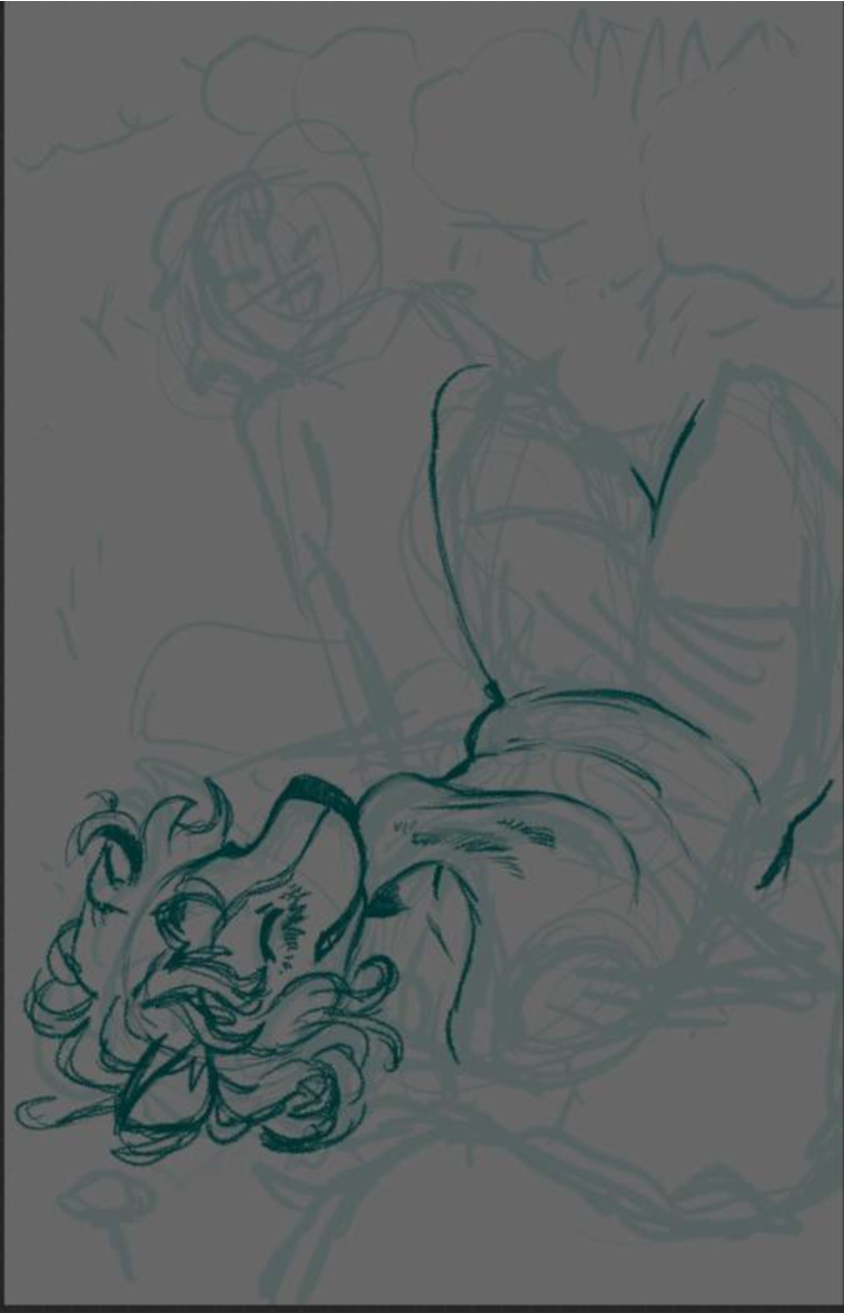
\includepdf[pages={1},noautoscale=true,fitpaper=true]{assets/ioanmay}}
Ioan made a face. ``I'd rather coffee.''

``I have no idea if the substitute was any good, but I like coffee, too.'' She held the flower up to her snout and smelled long at it. ``Me, though, I like the flowers. They are too complicated for their own good in this stage, are they not? Sure, they close up and then become the puffballs that spread them further and further, but here, they are almost platters of yellow.''

Ey grinned as she held the flower in both paws like a tray carrying food.

``But that is not what I like about them. I am telling you, now that you are awake, the things that I whispered to you to bring about this story. The things I suggested, as you put it. What I love is their scent.'' She held it up for em to sniff. ``They smell like muffins. How can anything that smells like muffins be bad? ''

Ey breathed deep of that scent. There was, indeed, the note of some baked sweet bread, but that was layered atop a vegetal scent. It was not unpleasant, but not precisely like a muffin. Ey decided not to share this opinion with May.

Instead, ey asked, ``Is that your story, May?''

``Of course not. You told the story yourself. Young Ioan with eir indoor lilacs.'' She laughed, peeking up at em slyly. ``Or perhaps we told the story. You asked, so I suggested, as you say, and you told the story.''

Ioan frowned, then rolled eir eyes. ``That's not what I asked, and you know it.''

``Tough shit. It is our story now,'' she said. ``Now, give me your hand.''

Ey held eir hand out for her, then let her turn it over in her paws. Before ey could object, she flipped the flower over, pressed it firmly to eir skin, and rubbed it in a vigorous circle.

``There.'' She held eir hand up so that ey could see, looking proud.

On the back of eir hand, the skin shone a golden yellow in the circle where she had rubbed the flower.

Ey shoved her over onto the grass, laughing. ``You nut.''

She lay there among the grass, giggling helplessly. Among the grass where a brand new dandelion poked through the green in front of her snout. One that had not been there before.
